\chapter{\textit{Mockup} da aplicação \textit{mobile}}
\label{Mockup}

Nas figuras \ref{mock1} e \ref{mock2} são apresentados os \textit{mockups} da aplicação \textit{mobile} prevista. 


\begin{figure}[h]
	\centering
	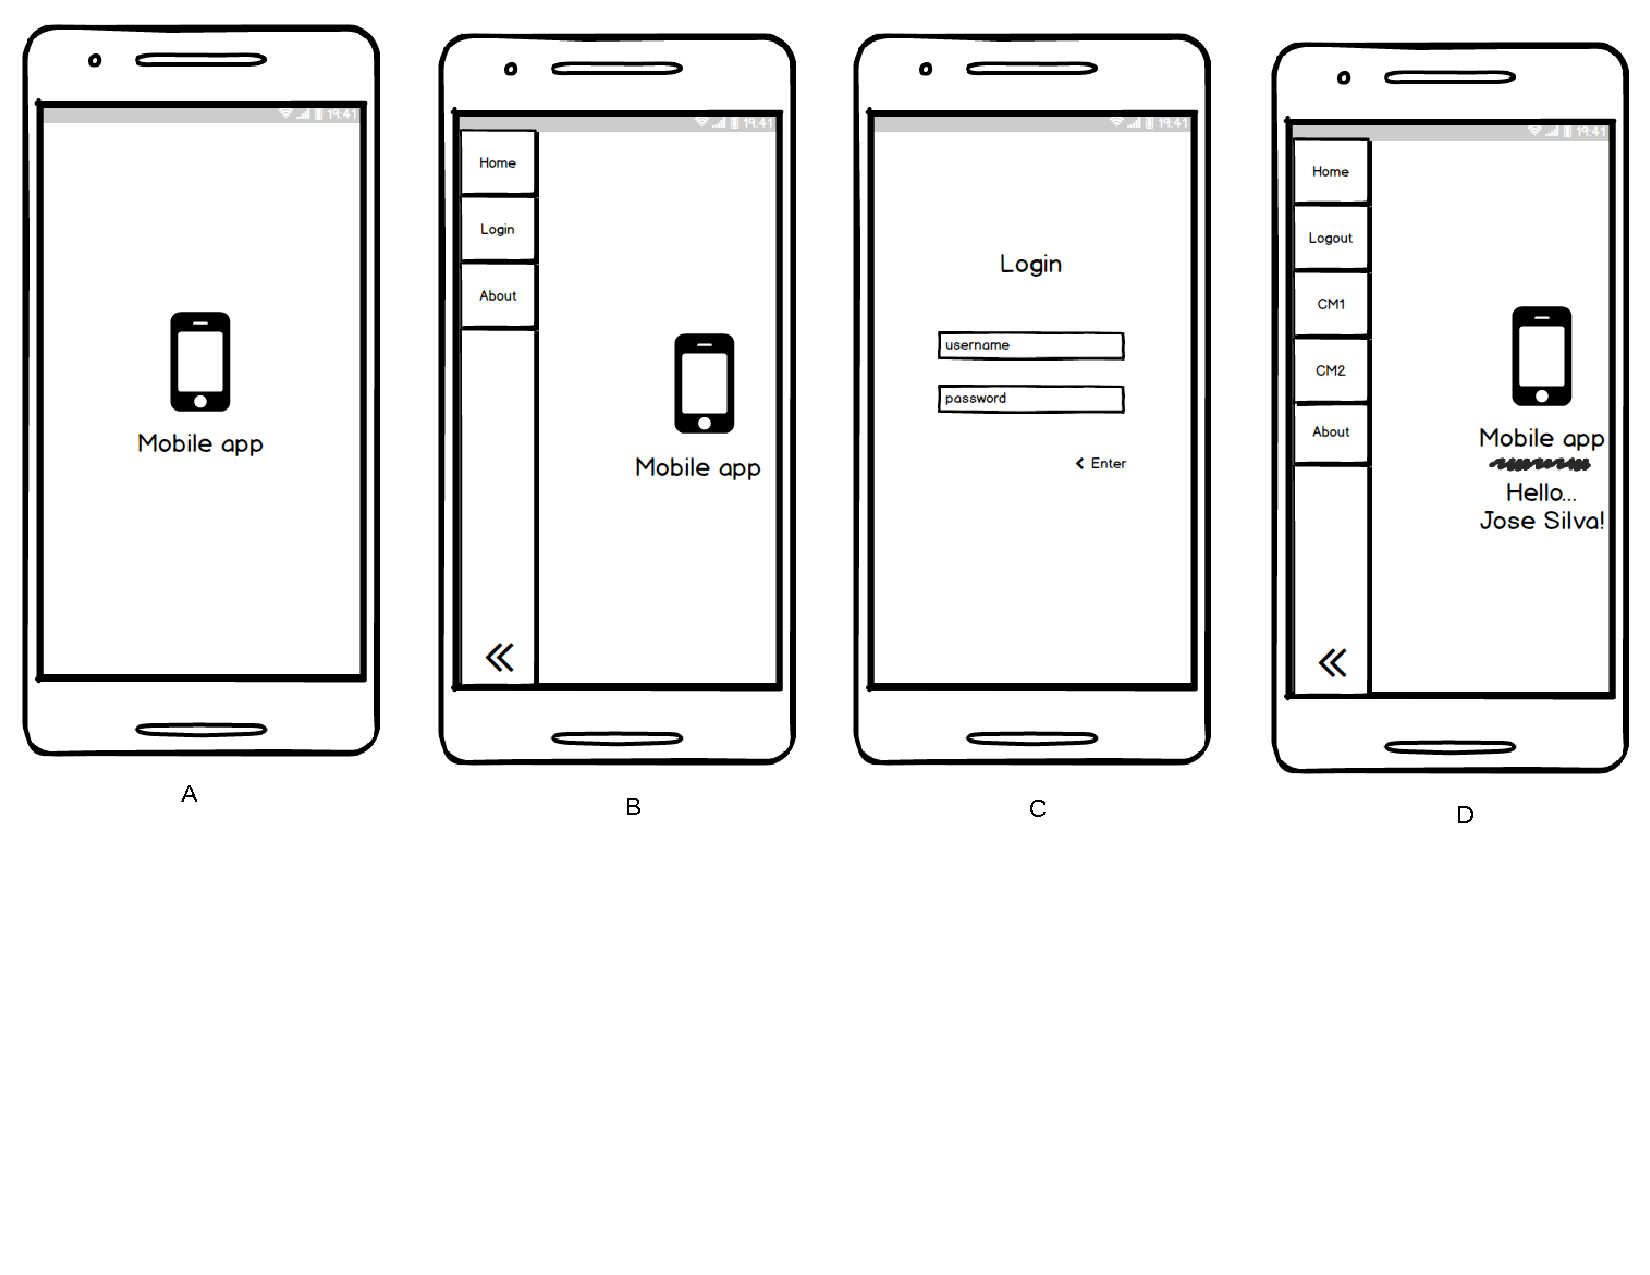
\includegraphics[width=\linewidth]{esquemas/mockup/1.pdf}
	\caption{\textit{Mockup} da aplicação \textit{mobile}}
	\label{mock1}
\end{figure}

\begin{itemize}
	\item \textbf{A}: página inicial da aplicação \textit{mobile}; 
	\item \textbf{B}: menu lateral deslizante (\textit{sidebar}) onde são apresentados os diferentes botões para as diferentes funcionalidades sem autenticação do utilizador; 
	
	\item \textbf{C}: página de \textit{login} na aplicação mobile; 
	\item \textbf{D}: página inicial e \textit{sidebar} após efecutar o \textit{login} do utilizador. 
\end{itemize}


\newpage


\begin{figure}[h]
	\centering
	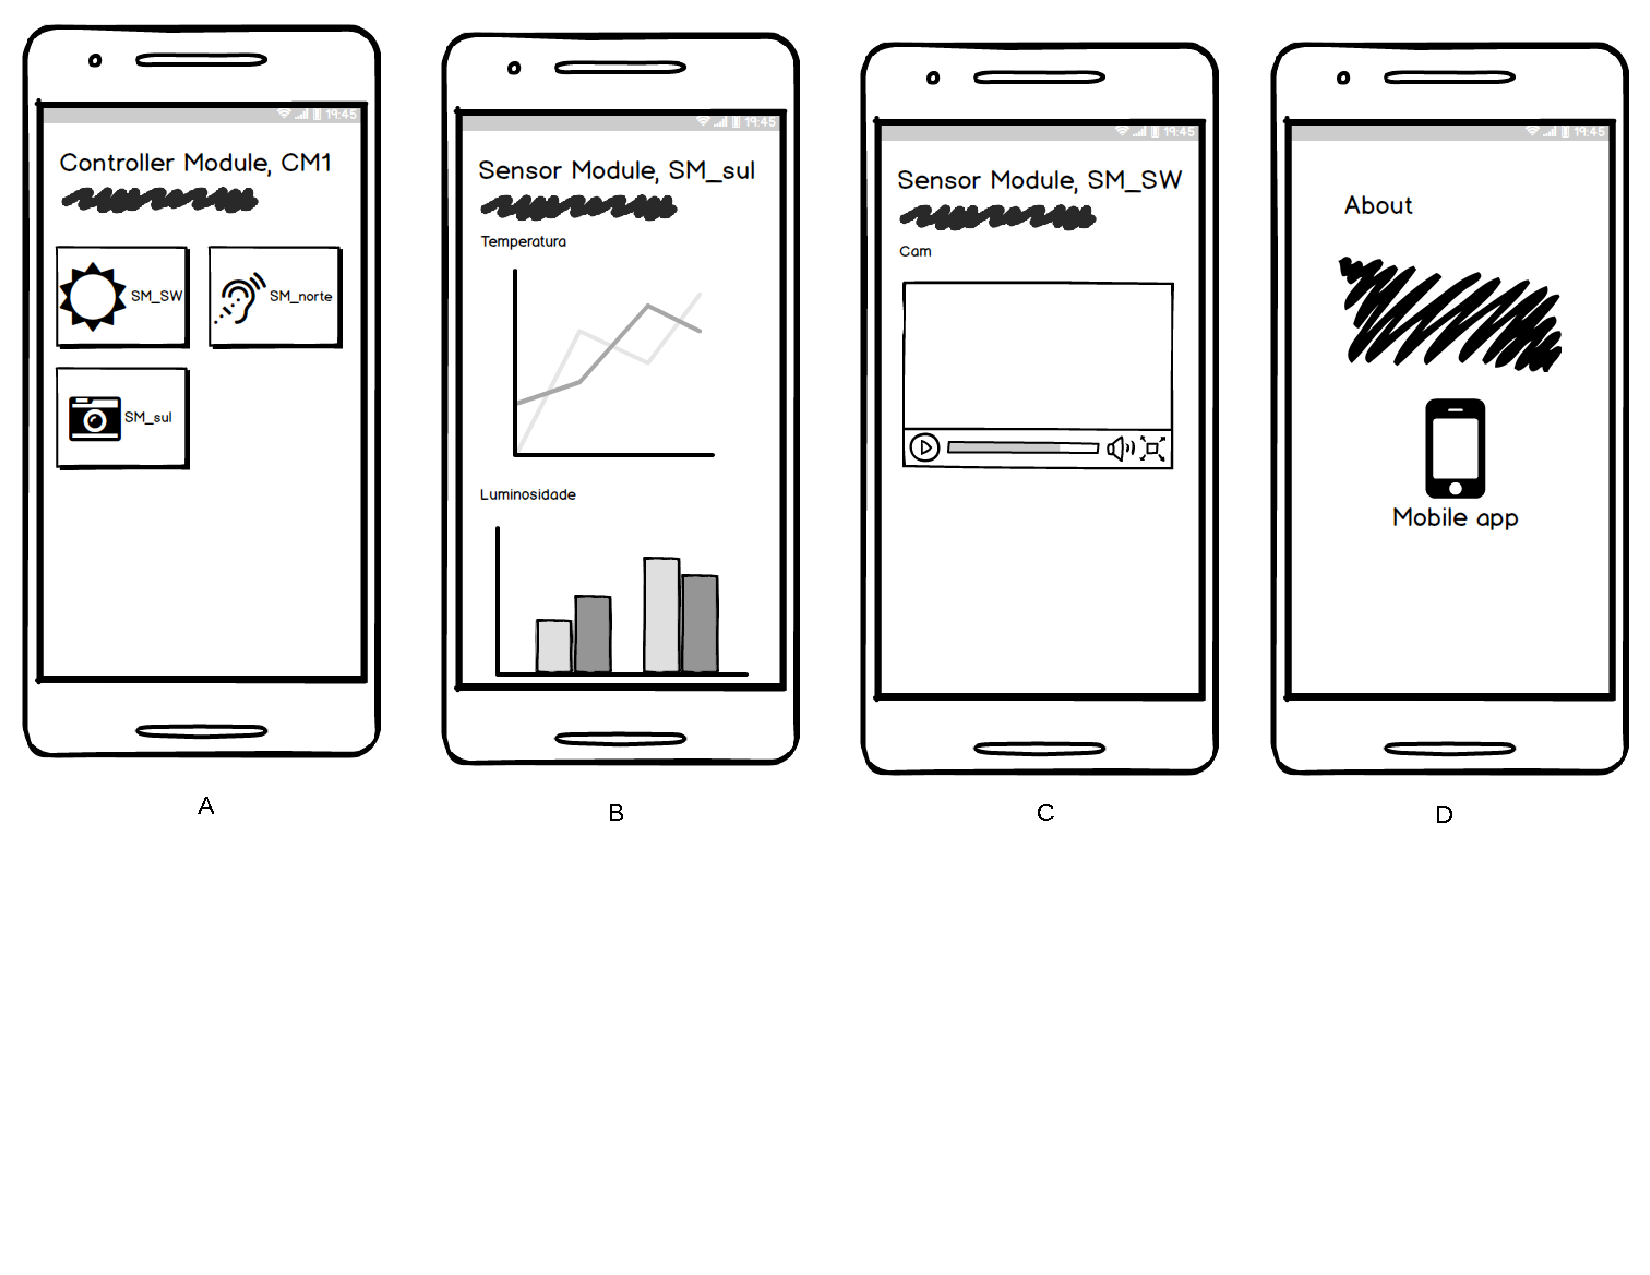
\includegraphics[width=\linewidth]{esquemas/mockup/2.pdf}
	\caption{\textit{Mockup} da aplicação \textit{mobile} (continuação)}
	\label{mock2}
\end{figure}

\begin{itemize}
	\item \textbf{A}: página de detalhes de um \acl{CM}, onde são apresentados os botões para cada \acl{SM} existente; 
	\item \textbf{B}: página de detalhes de um \acl{SM}, onde são apresentados os dados adquiridos pelos sensores em modo gráfico; 
	\item \textbf{C}: página para visualização do sistema de video-vigilância; 
	\item \textbf{D}: página de informações da aplicação.
\end{itemize}